\documentclass[11pt]{report}
\usepackage[pdftex]{graphicx}

\usepackage{henrian-basic}
\usepackage{henrian-homework}

\usepackage{amsmath}
\usepackage{float}

\makeHeaders{Machine Learning: Homework 7}

\tolerance=100000

\begin{document}

\begin{itemize}
  \item \textbf{Email}: chrisbrown@utexas.edu
  \item \textbf{EID}: chb595
\end{itemize}

\section{Q-learning}

\subsection{Enviroment}


\begin{figure}[H]
  \centering
  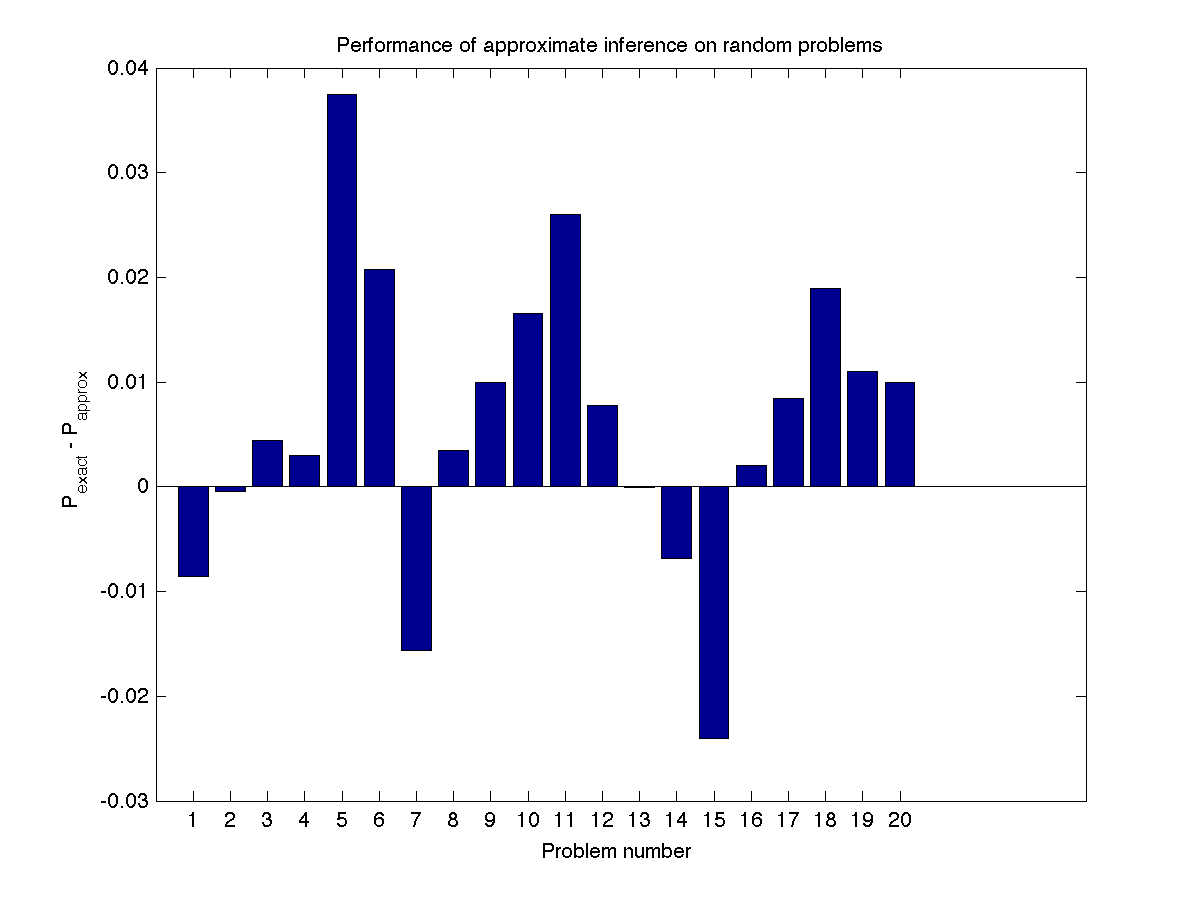
\includegraphics[width=0.95\textwidth]{hw6-plot-n1000.png}
  \caption{.}
  \label{fig:n1000}
\end{figure}


\begin{figure}[H]
  \centering
  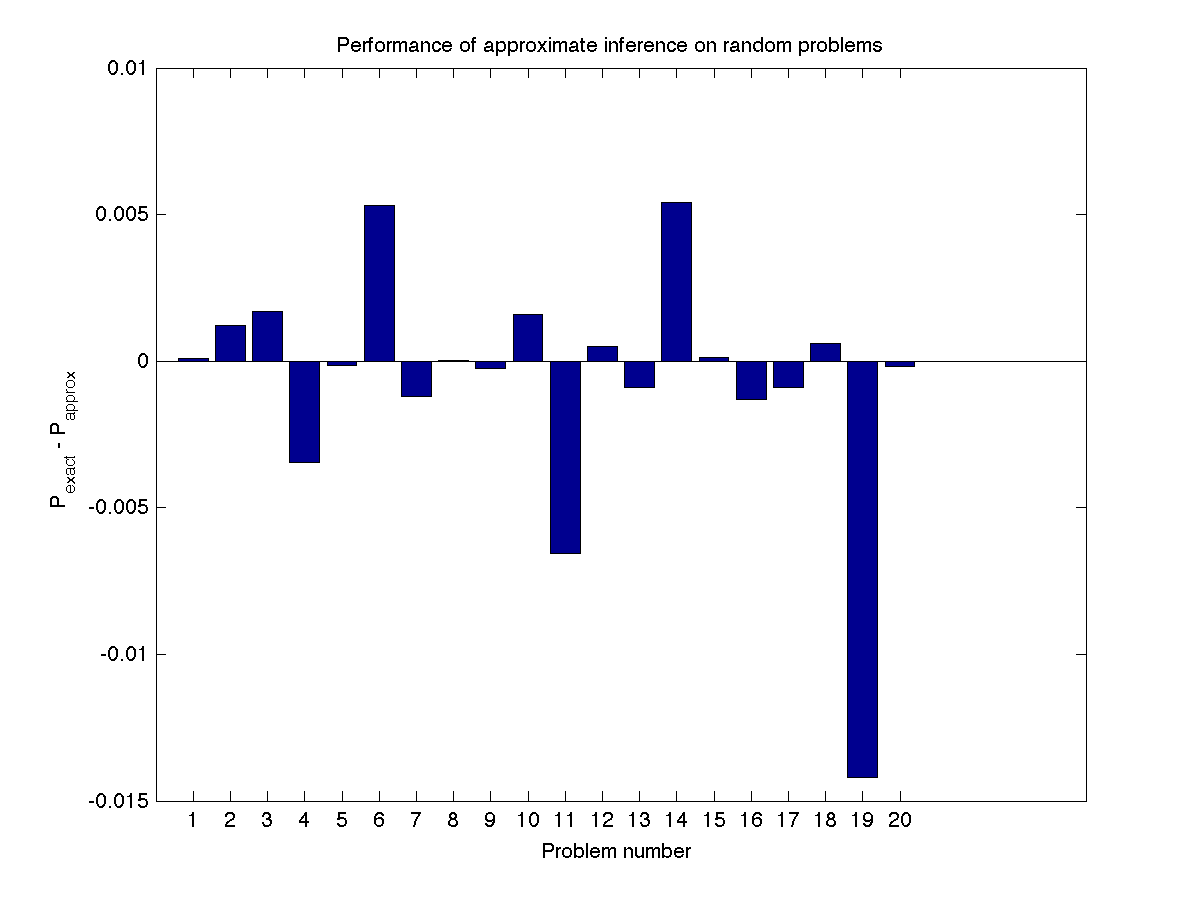
\includegraphics[width=0.95\textwidth]{hw6-plot-n10000.png}
  \caption{.}
  \label{fig:n10000}
\end{figure}

\noindent In Figure \ref{fig:n10000}, 

\begin{figure}[H]
  \centering
  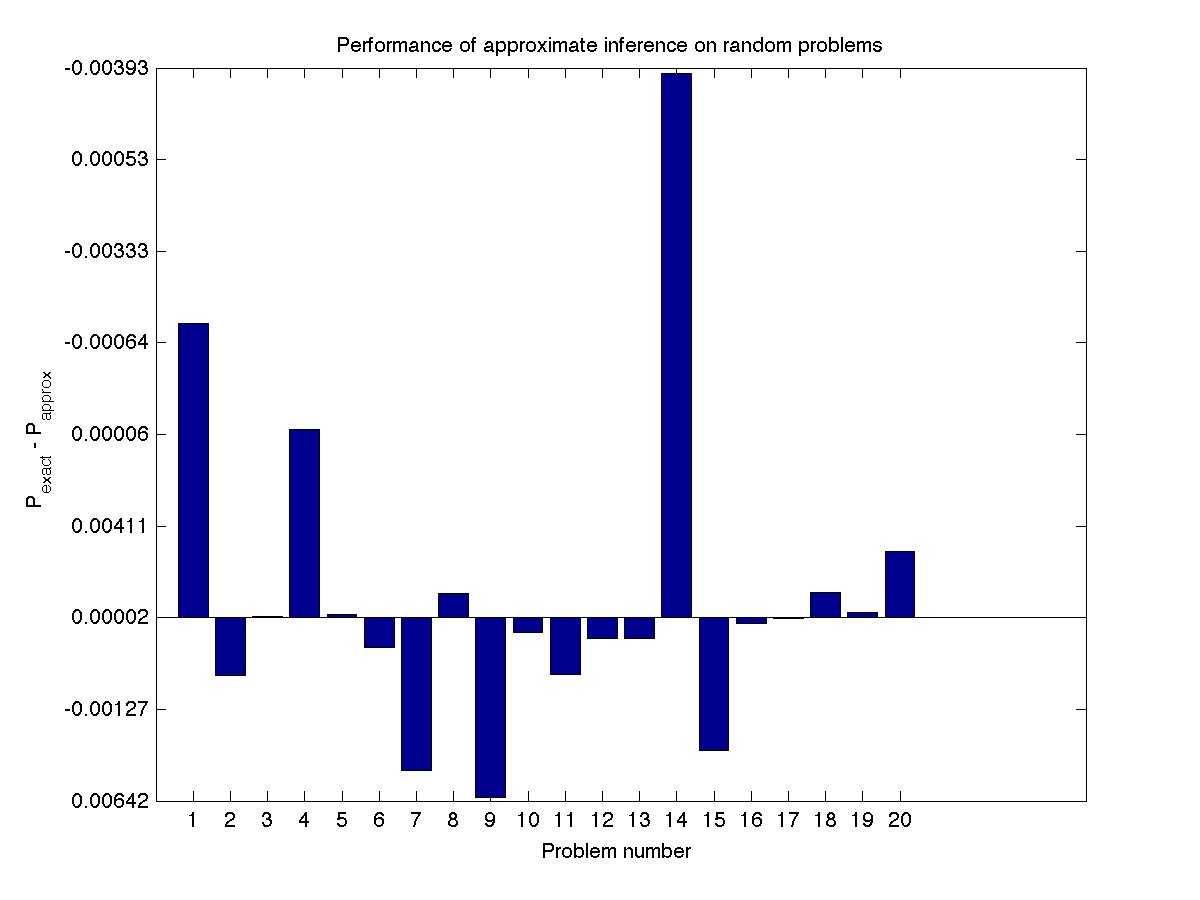
\includegraphics[width=0.95\textwidth]{hw6-plot-n10000-burnin.png}
  \caption{.}
  \label{fig:n10000-burnin}
\end{figure}

\section{Pitfalls}

There were a couple of hacks that I had to build into my algorithm:
\begin{enumerate}[a.]
  \item Often in the very first runs of the \texttt{finish} module, the agent would jitter left and right while running the width of the sidewalk several times, not making any forward progress. As far as I can tell, this was due to tiny differences between the score for going left as opposed to right, in the range of $< 0.0001$. Of course, sorting will register tiny differences just as significant as more reasonable (0.5) differences, so my hack was to pick a random action if the advantage between choosing the best and the worst 

  I could have accomplished the same thing by adding a very amount of noise, e.g. $\mathcal{N}(0, 0.00001)$, to the Q function, but the threshold solution was easier and faster.


\end{document}
